

\section{Evaluation}
\label{sec:eval}
%
Lorem ipsum dolar sit amat

\begin{figure*}[t]
	{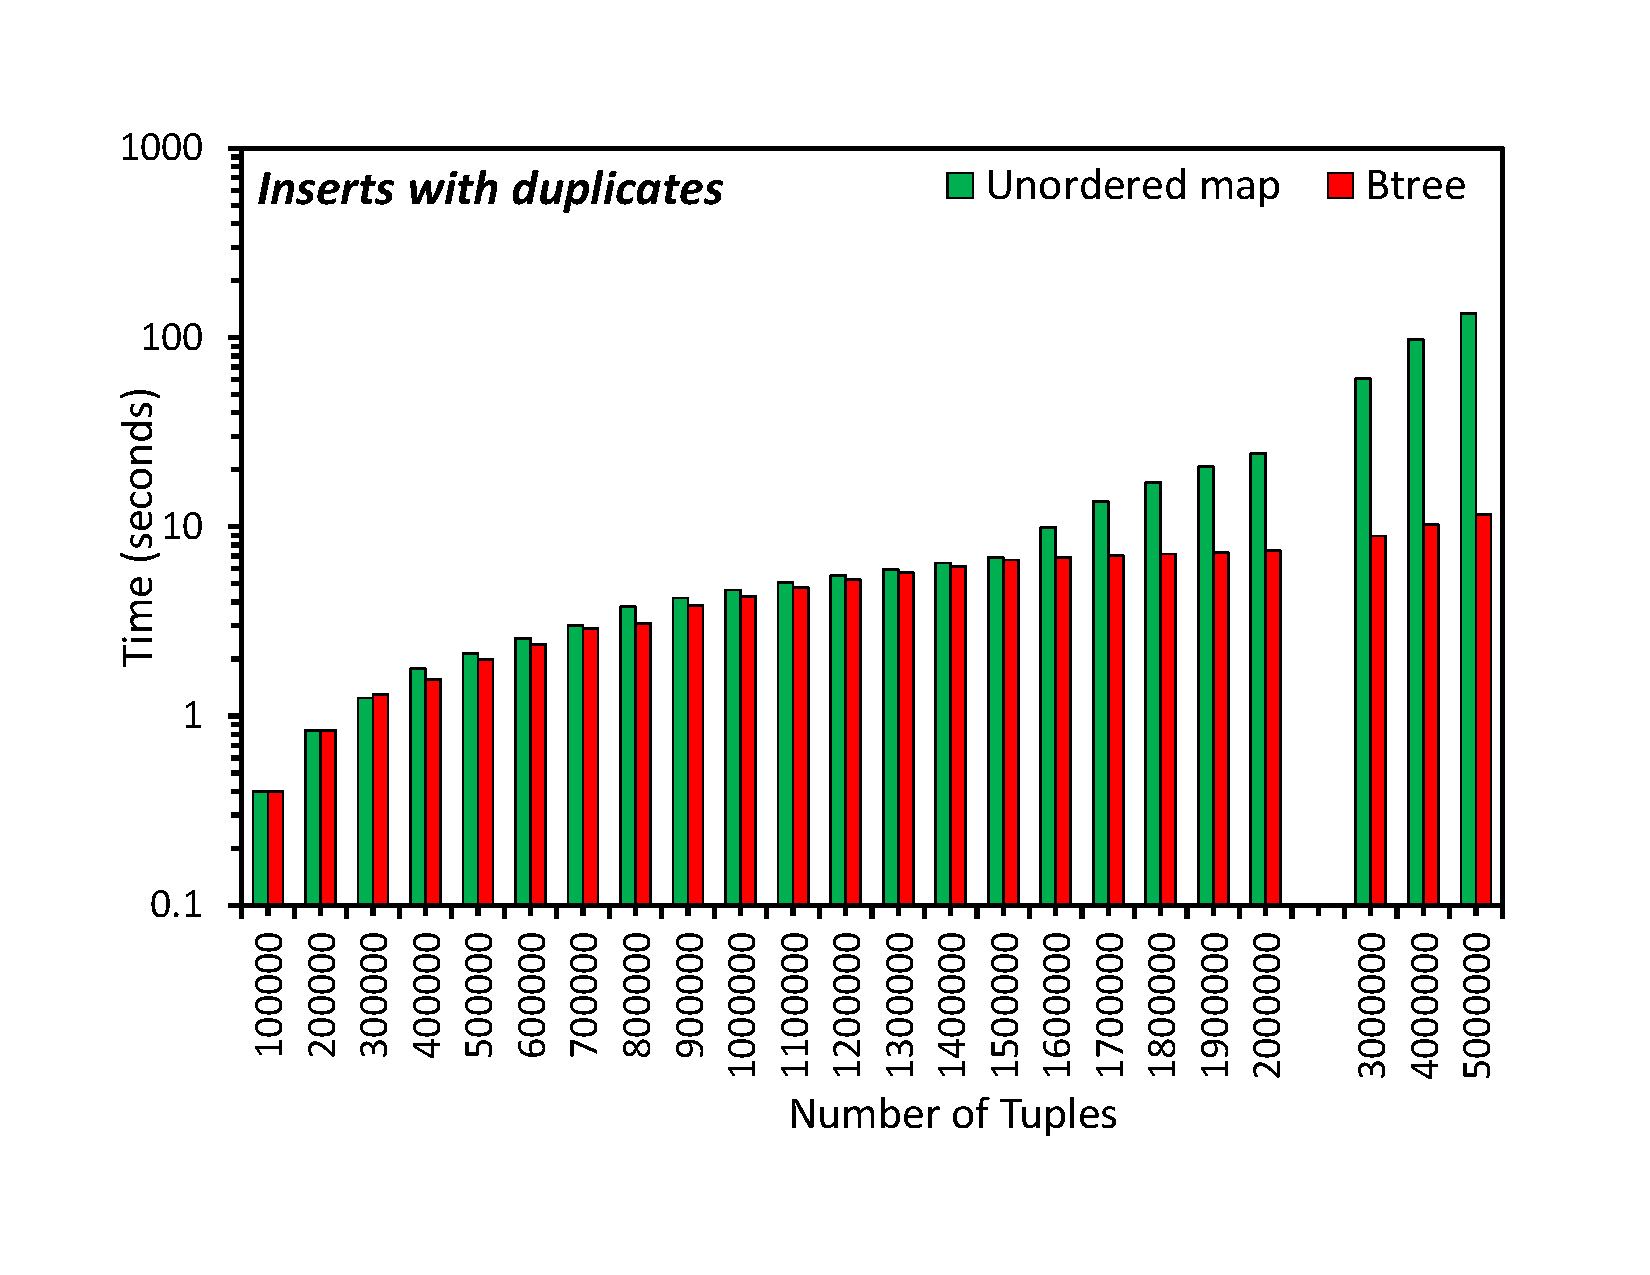
\includegraphics[width=.50\textwidth,  trim={0cm 0cm 0cm 0cm, 
			clip}]{results/inserts_with_duplicates.pdf}}\hfill%
	{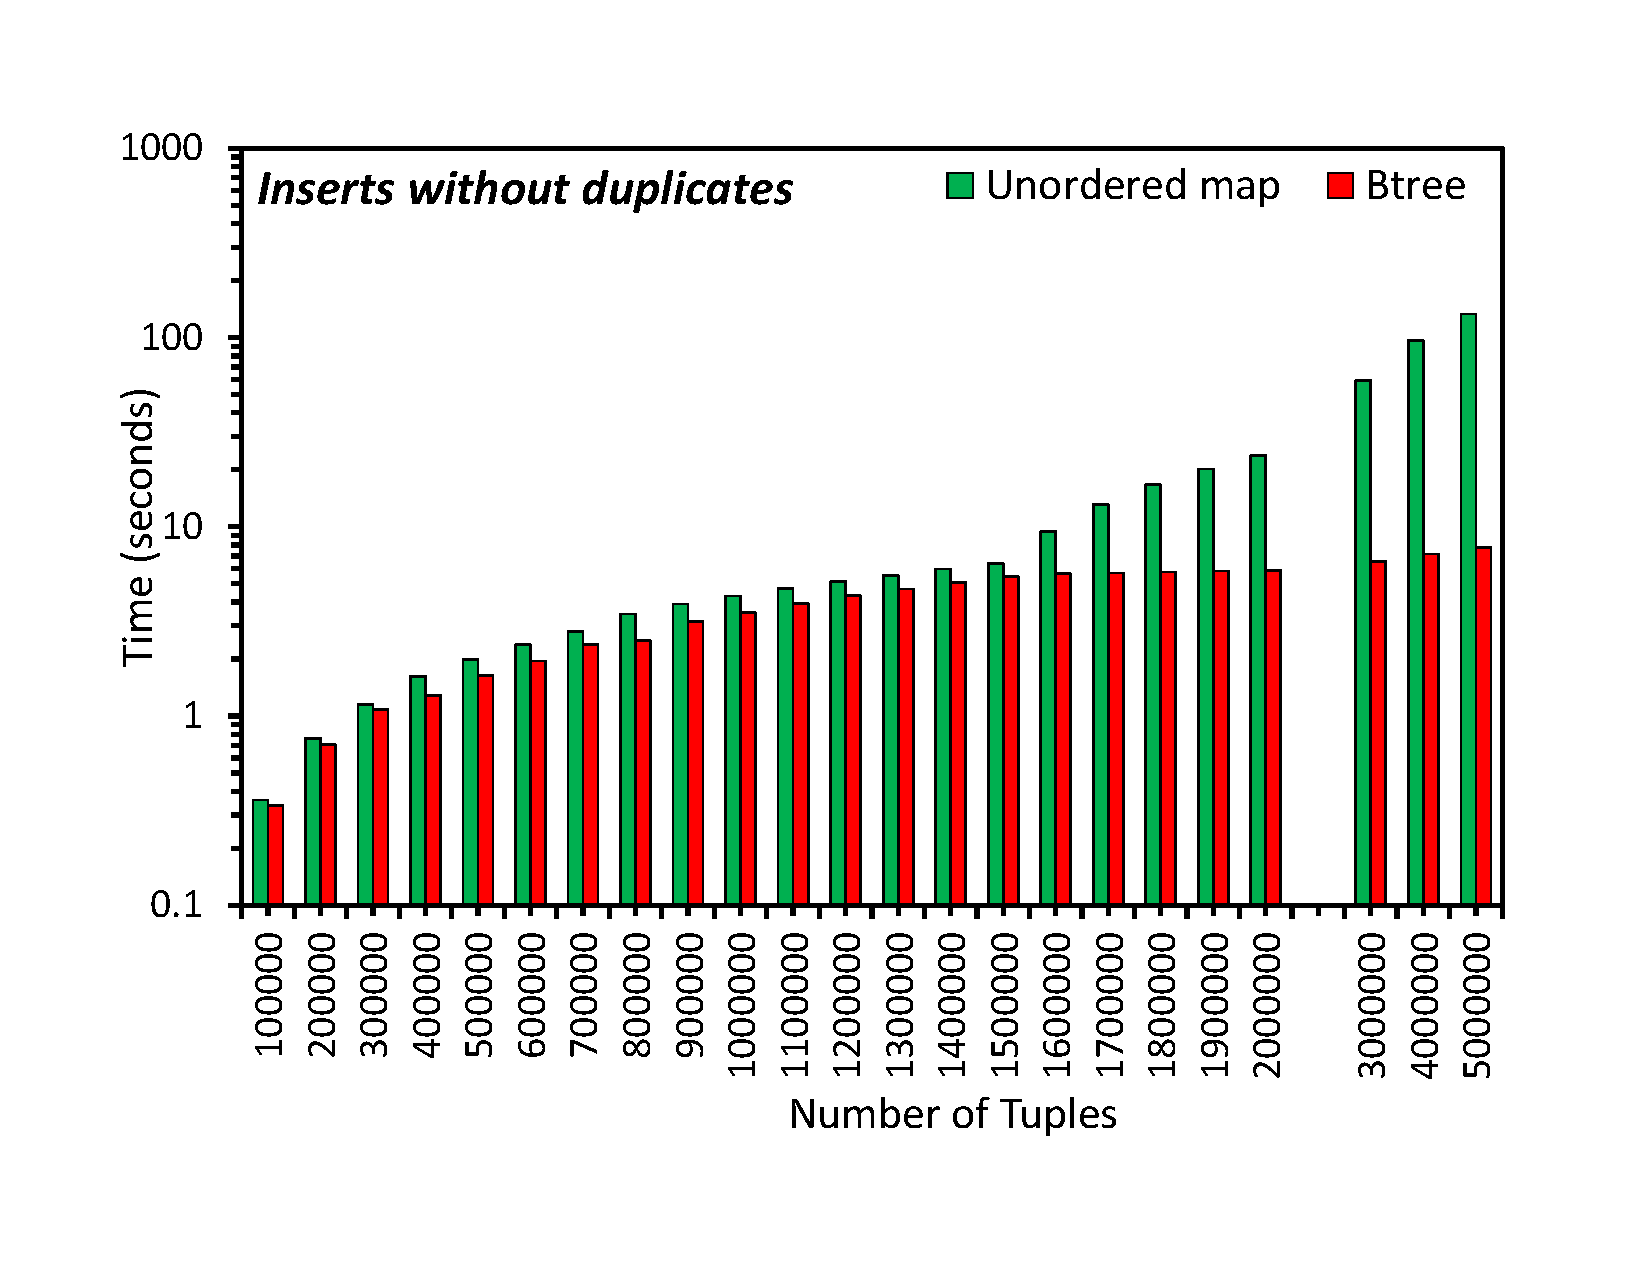
\includegraphics[width=.50\textwidth,  trim={0cm 0cm 0cm 0cm,
			clip}]{results/inserts_with_no_duplicates.pdf}}\hfill%
	\centering
	\caption{Performance evaluation of relation class implemented with btree and unordered map. (left) All tuples are distinct, (right) There are four copies of every tuple being inserted. Relation implemented with btree out-performs the unordered-map implementation.}
	\label{fig:tuple_inserts}
\end{figure*}


\begin{figure*}[t]
	{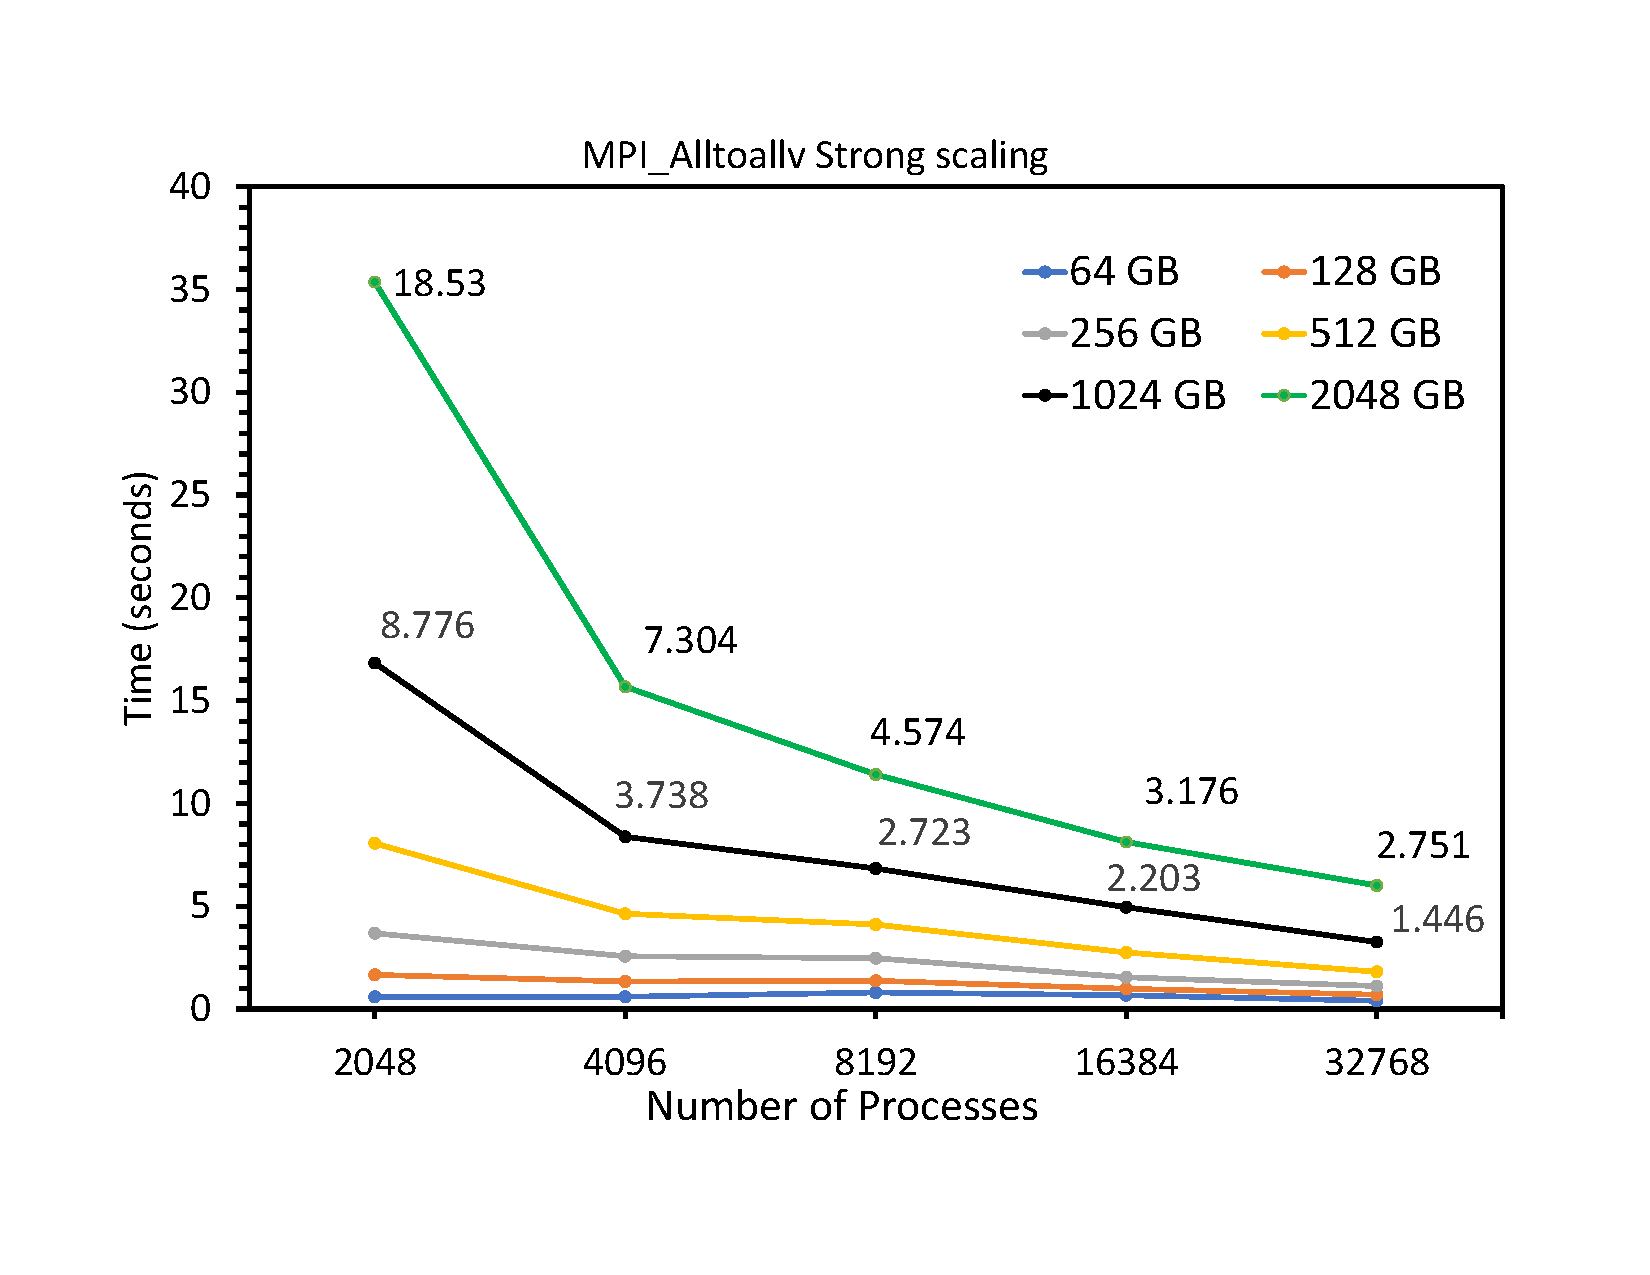
\includegraphics[width=.50\textwidth,  trim={0cm 0cm 0cm 0cm, 
			clip}]{results/all_to_all_strong.pdf}}\hfill%
	{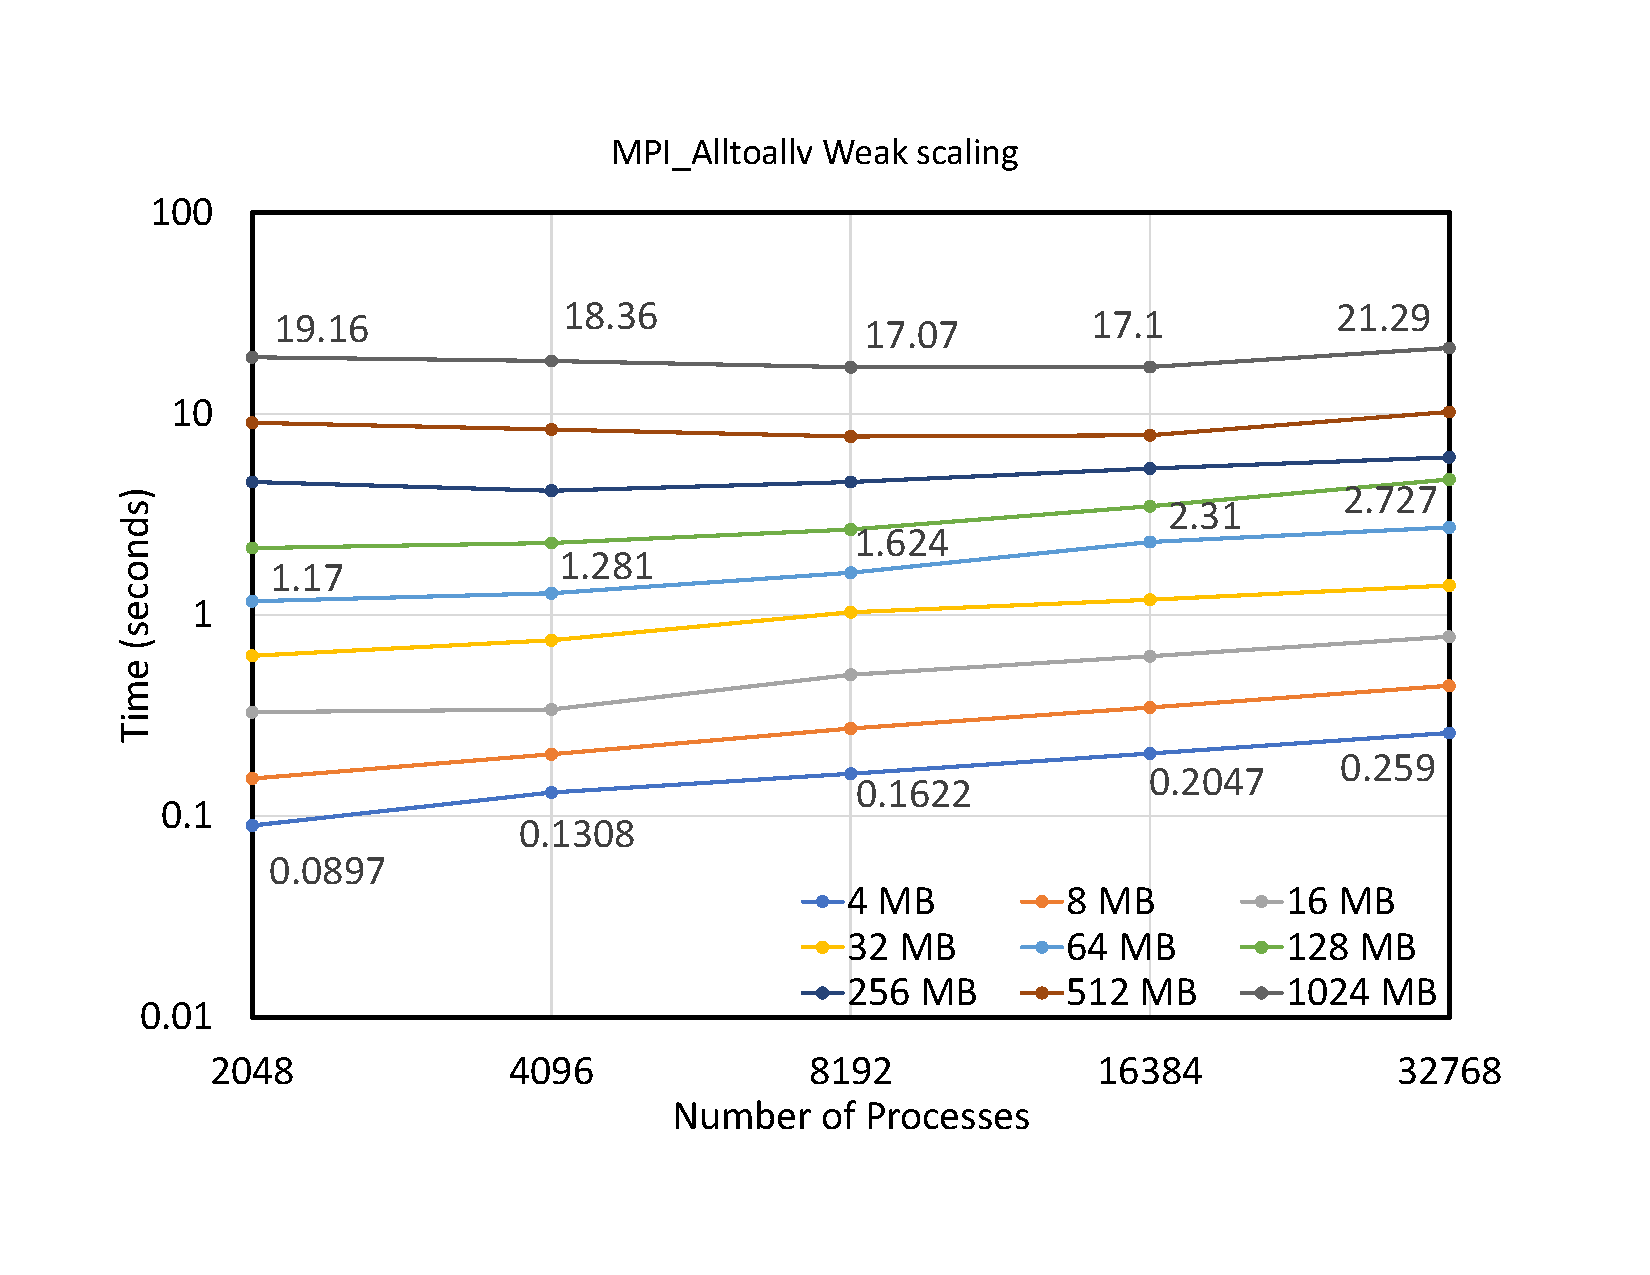
\includegraphics[width=.50\textwidth,  trim={0cm 0cm 0cm 0cm,
			clip}]{results/all_to_all_weak.pdf}}\hfill%
	\centering
	\caption{Strong (left) and Weak (right) scaling evaluation of MPI\_alltoallv function of MPI.}
	\label{fig:all_to_all}
\end{figure*}


\begin{figure*}[t]
	{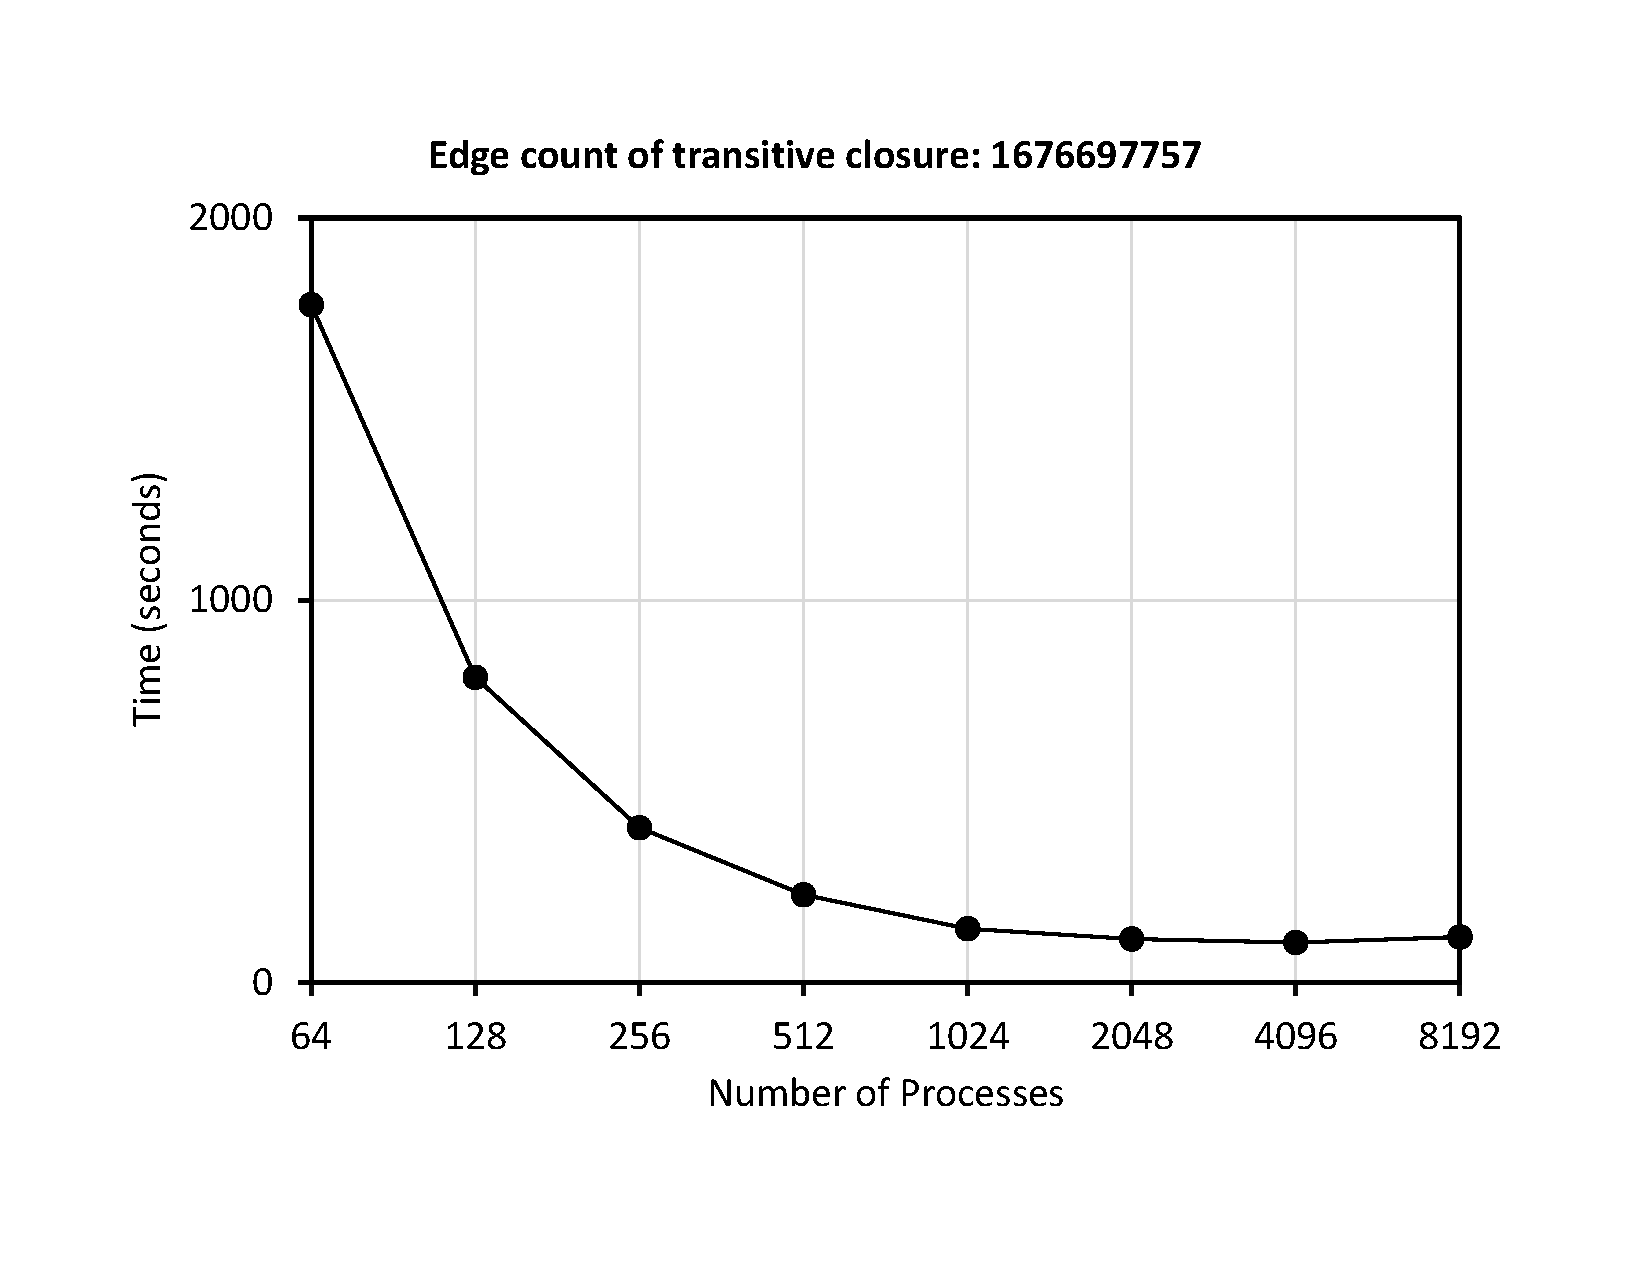
\includegraphics[width=.50\textwidth,  trim={0cm 0cm 0cm 0cm, 
			clip}]{results/TC_1_6Billion.pdf}}\hfill%
	{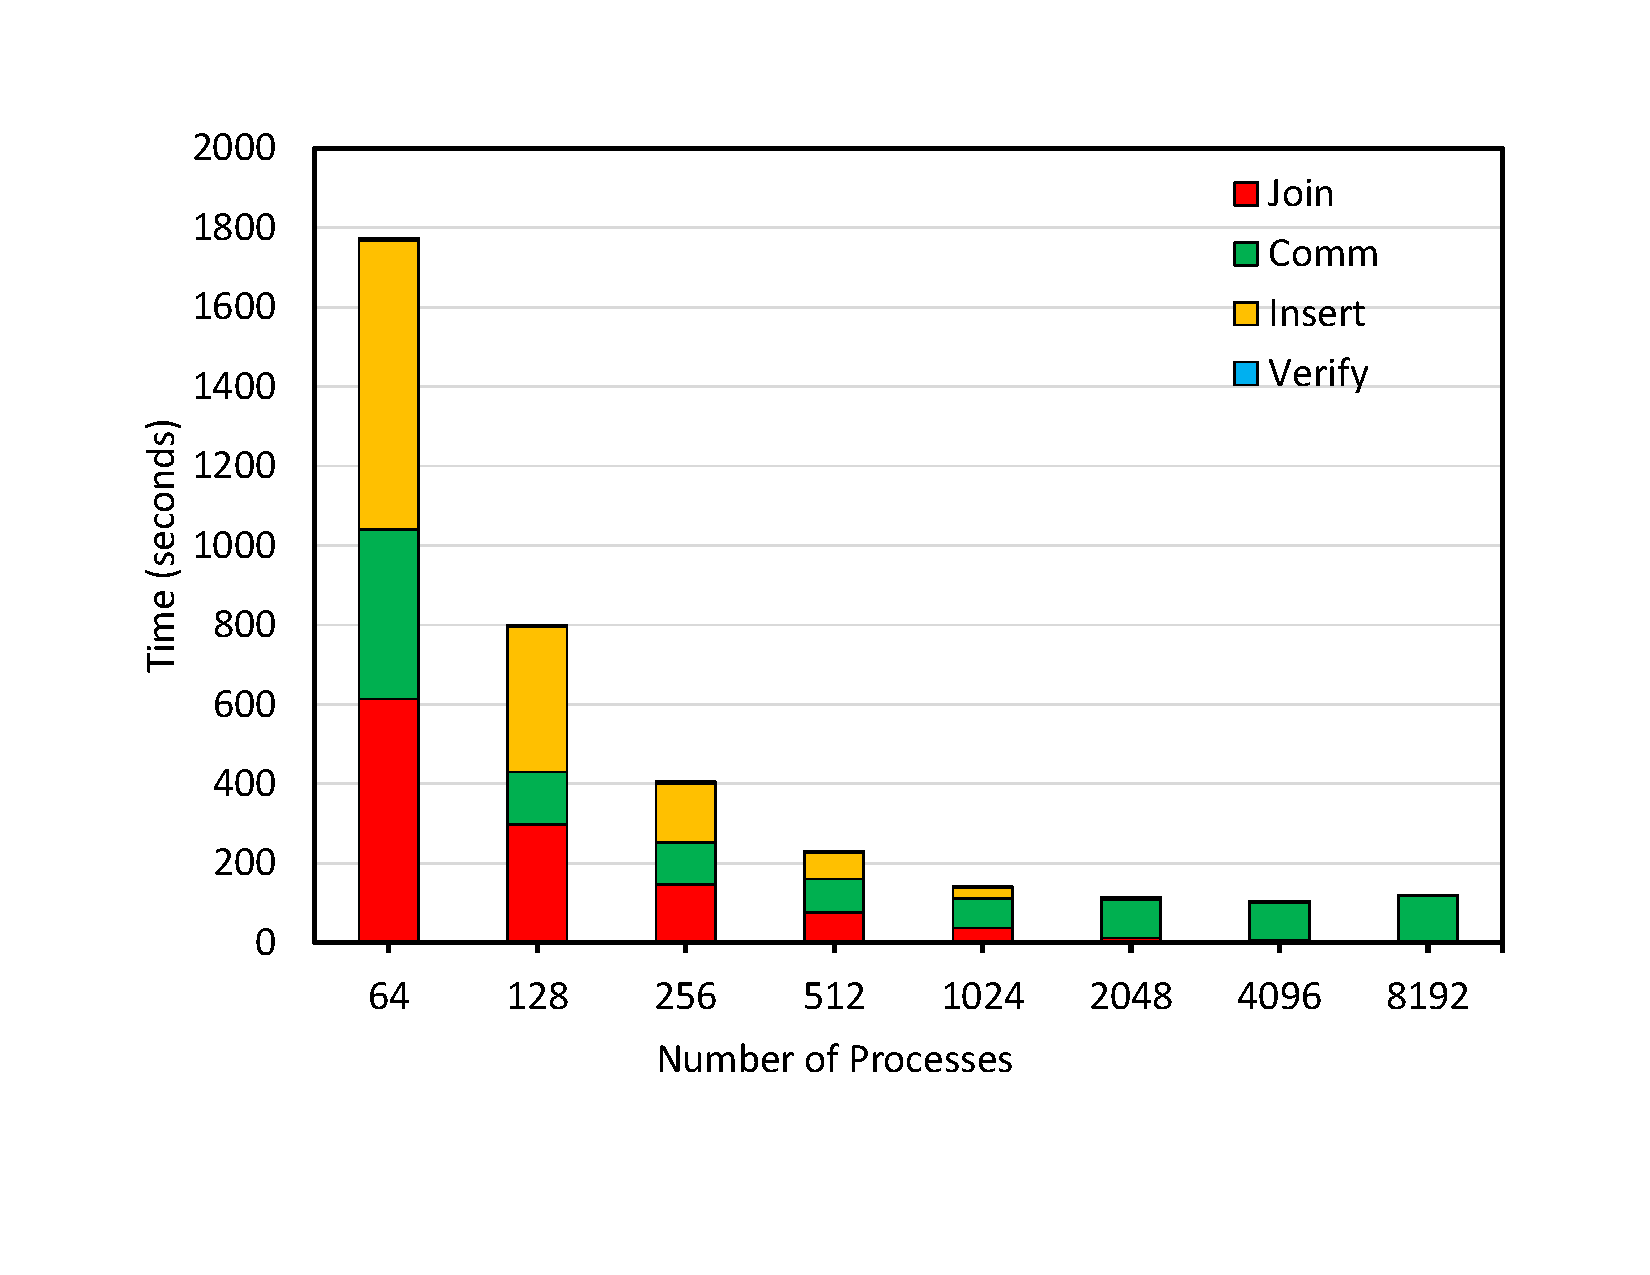
\includegraphics[width=.50\textwidth,  trim={0cm 0cm 0cm 0cm,
			clip}]{results/TC_1_6Billion_breakdown.pdf}}\hfill%
	\centering
	\caption{Transitive closure of a graph with X edges.}
	\label{fig:tc_small}
\end{figure*}


\begin{figure*}[t]
	{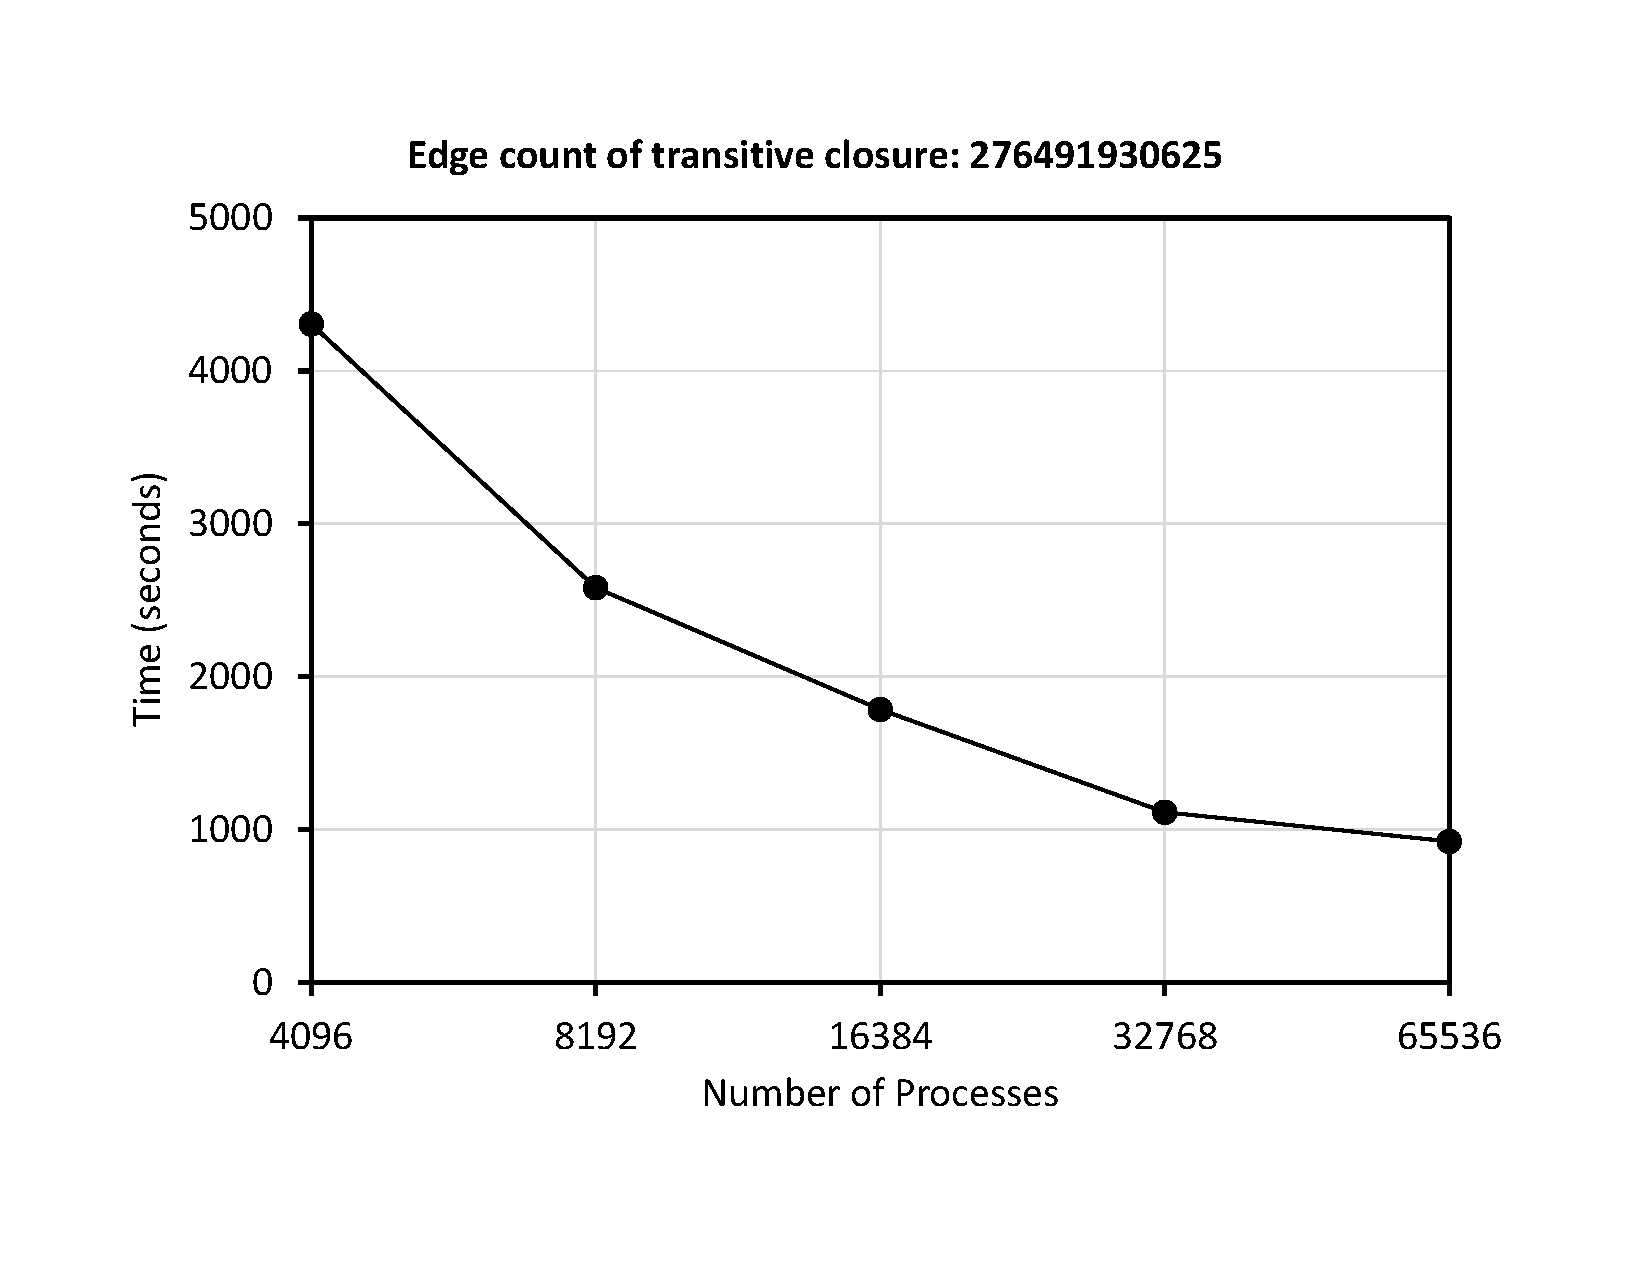
\includegraphics[width=.50\textwidth,  trim={0cm 0cm 0cm 0cm, 
			clip}]{results/TC_260Billion.pdf}}\hfill%
	{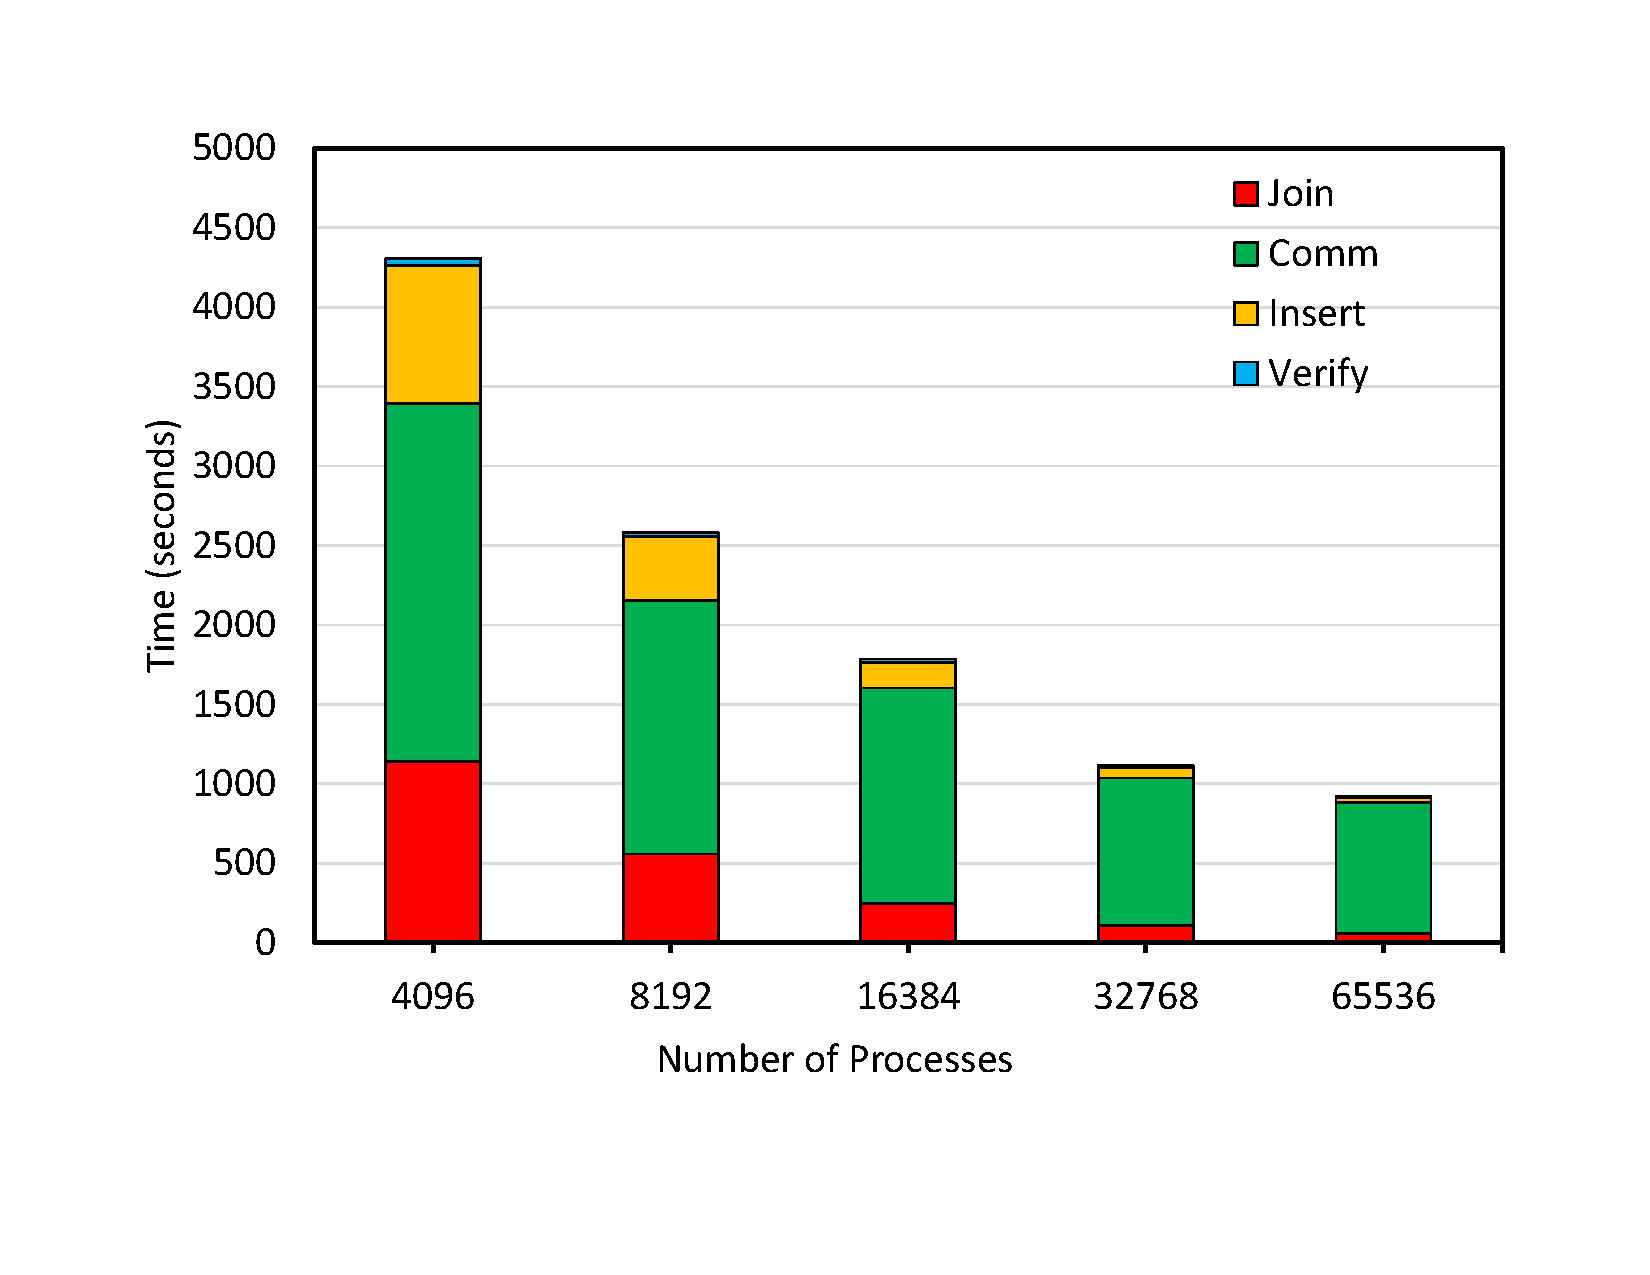
\includegraphics[width=.50\textwidth,  trim={0cm 0cm 0cm 0cm,
			clip}]{results/TC_260Billion_breakdown.pdf}}\hfill%
	\centering
	\caption{Transitive closure of a graph with X edges.}
	\label{fig:tc_large}
\end{figure*}